\chapter{Modelo de minería de datos clínicos y genómicos}

La importancia de la minería de datos clínicos y genómicos radica en el diseño e implementación de modelos que permitan la extracción de información relevante de datos clínicos y genómicos, para transformarlos en conocimiento, y que sean aplicables a las investigaciones y procesos diagnósticos \cite{Farid2016}. \\  

Este capítulo presenta el diseño y la implementación de un modelo de minería aplicado que permita la asociación entre las variantes identificadas en regiones codificantes de genes con datos clínicos en pacientes colombianos.El capítulo presenta un análisis descriptivo de datos clínicos y variantes de los datos,un análisis textual de información clínica,una asociación de grupos con variantes, una propuesta de visualización,discusión, conclusiones y resumen. 

\section{Diseño del modelo de minería de datos}

La selección de las tareas de minería a realizar se dio por la necesidad de caracterizar los fenotipos de los individuos a partir de la información clínica y para poder realizar esta tarea fue necesario realizar procesamiento de lenguaje natural de dicha información para poder generar grupos de pacientes. En cuanto las variantes se utilizo reglas de asociación para poder aprovechar las frecuencias de las variantes y a que otras características pueden estar asociadas.El modelo de minería de datos esta representado por la figura  \ref{fig:kdd}:\\

\begin{figure}[H]
	\centering
	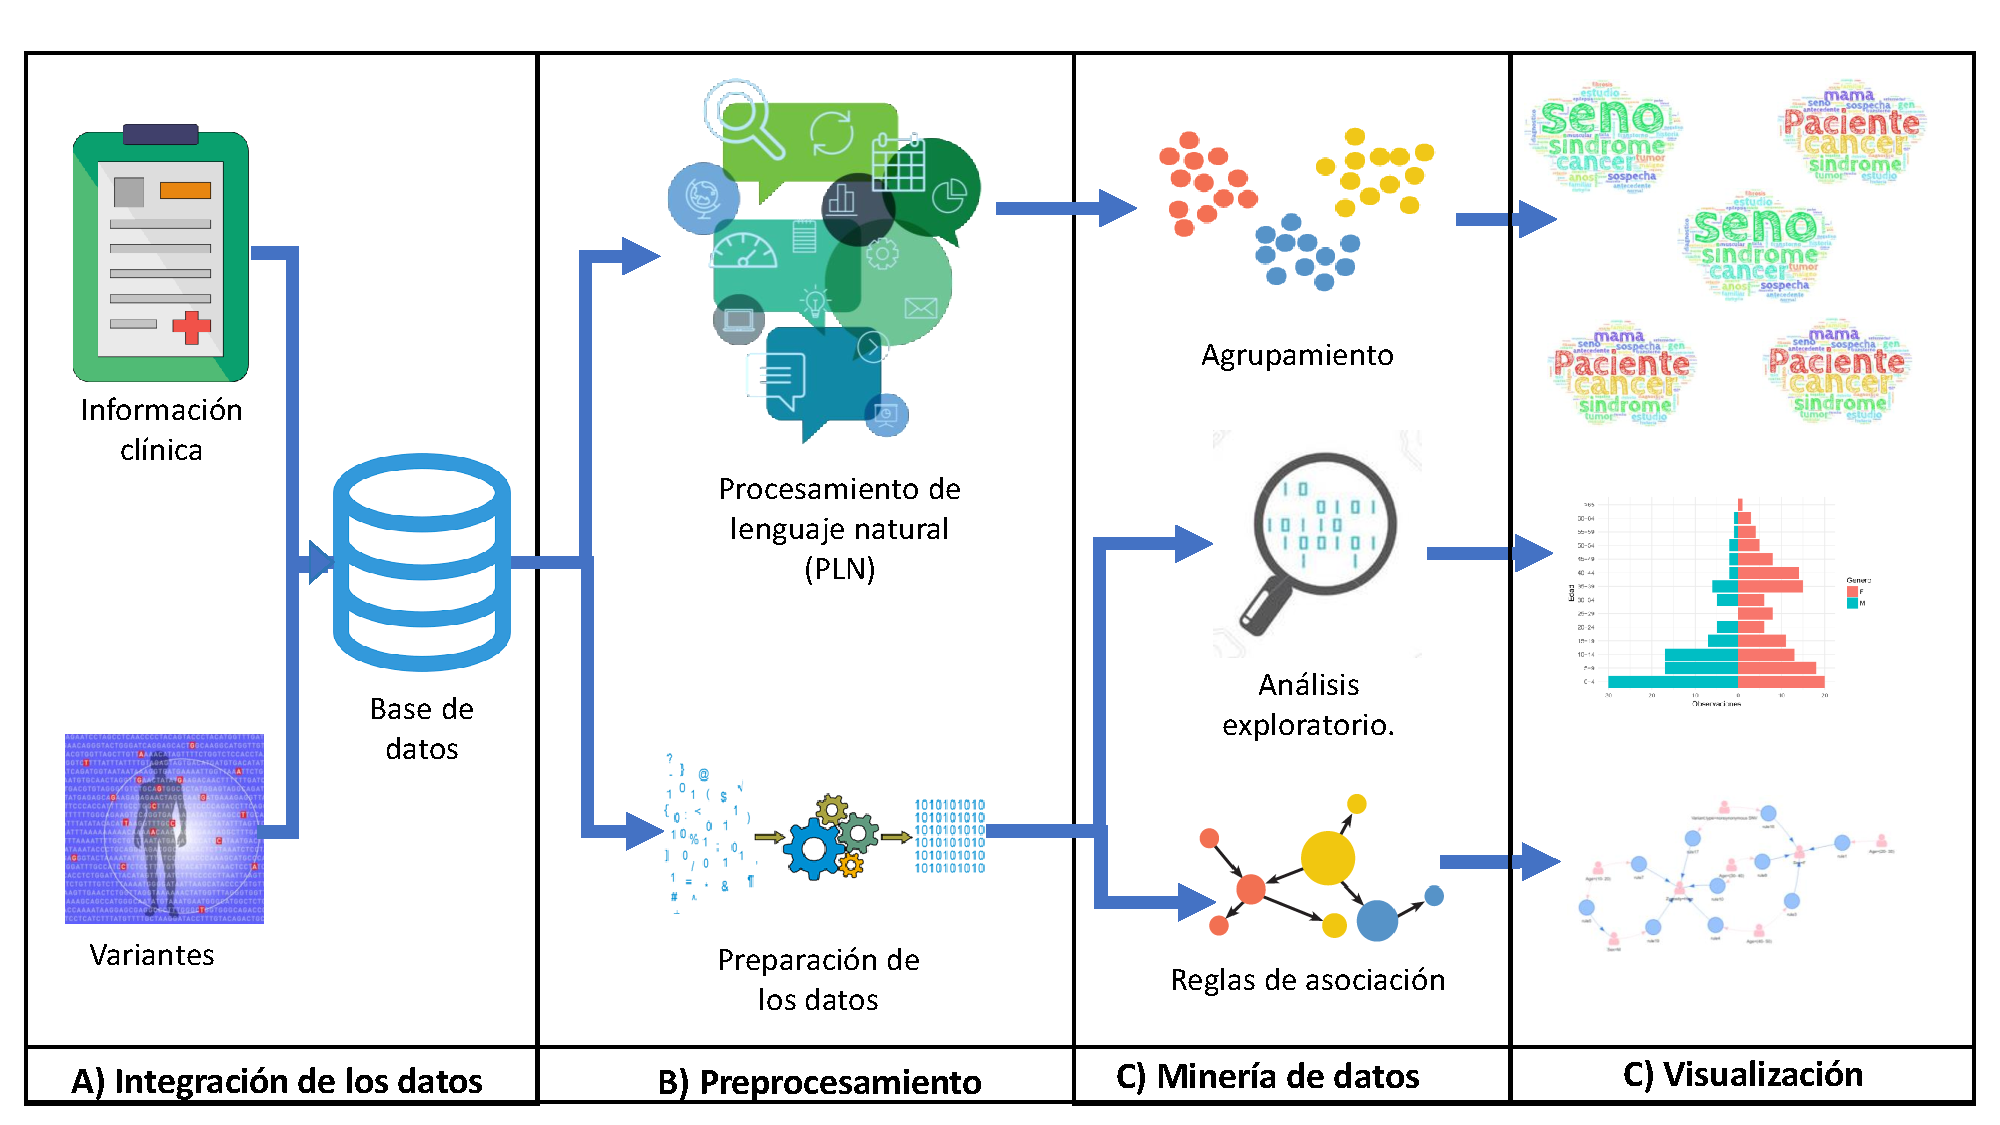
\includegraphics[width=0.8\textwidth]{Kap4/KDDtesis.pdf}
	\caption{Modelo de minería de datos}
	\label{fig:kdd}
\end{figure}


 La figura \ref{fig:kdd} se divide en partes que son una representación gráfica de como se diseño el modelo de minería en la  parte A) Resume la integración de datos que se realizo en el capitulo anterior. B) Muestra que la información integrada se proceso de forma separada pero paralela, se tiene un procesamiento de lenguaje natural de la información clínica disponible, y una preparación de las variantes para ser asociadas. C) Muestra el proceso de minería de datos, en el cual se realiza el análisis exploratorio de los datos después de haber sido preprocesados, y la aplicación de las técnicas del modelo de minería que fueron agrupamiento de la información clínica y reglas de asociación para las variantes. Finalmente la parte D) muestra la propuesta para la visualización de los resultados en cuál se encuentran las nubes de palabras de los grupos obtenidos después de realizar el agrupamiento, un ejemplo de los resultados del análisis exploratorio y un ejemplo de la visualización de reglas de asociación de las variantes.



\section{Análisis exploratorio de datos clínicos y variantes}

Se presenta un análisis de los datos clínicos  y genómicos de los pacientes depositadas en la base de datos presentada en el capítulo anterior. Este análisis se realiza en los datos como son la edad, genero y tipos de variantes. La base de datos contiene 228 pacientes de los cuales 133 son de género femenino y tienen un total de 468.485 variantes y 95 pacientes de género masculino con 345.239 de variantes obteniendo  un total de 803.878 variantes. La  figura \ref{fig:general} representa la distribución de pacientes por rango de edades.\\

\begin{figure}[h]
	\centering
	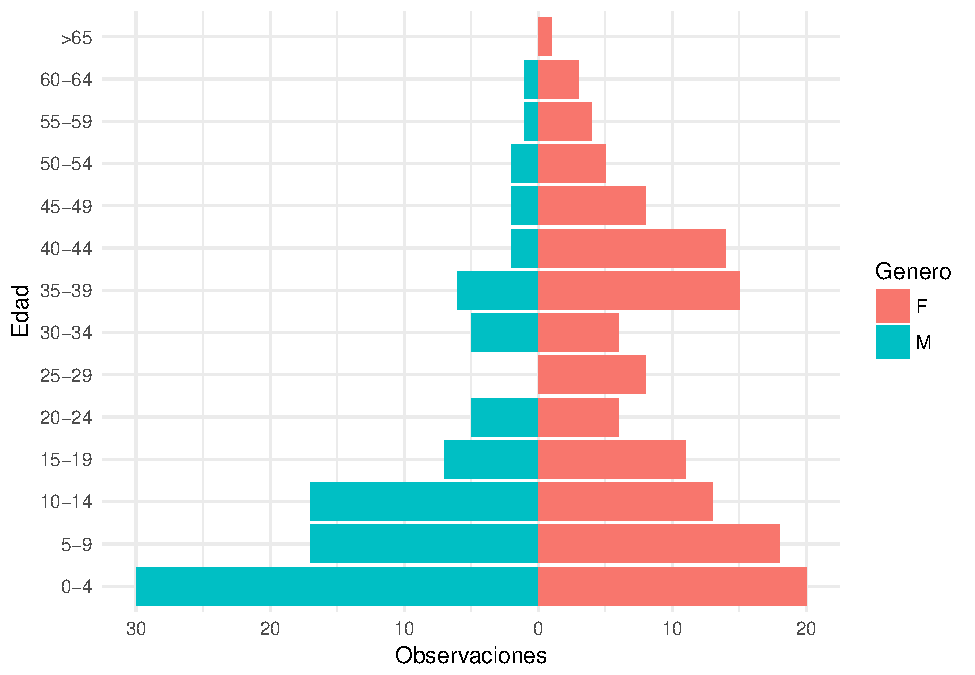
\includegraphics[width=0.6\textwidth]{Kap4/general}
	\caption{Distribución de rango de edades y géneros de los pacientes}
	\label{fig:general}
\end{figure}

La figura \ref{f:variantesgeneral}(a) representa la distribución de variantes según su tipo. En la figura \ref{f:generosgeneral}(b) muestra la distribución  de variantes, donde las variantes que son sinónimas y no sinónimas las más frecuentes en la población, a  nivel mundial se conoce que estos son lo tipos de variantes más frecuentes\cite{Fu2013}.Las variantes ``unknown"  son el tercer tipo de variante más frecuente dado que aún existe el problema de selección del transcripto para realizar la nomenclatura adecuada de las variantes, por lo que el anotador informa que son desconocidas \cite{McCarthy2014}.\\

 La figura\ref{f:variantedad} muestra la distribución de las variantes identificadas según el rango de edad, siendo el rango con mayor número de variantes los pacientes que se encuentran entre las edades de 0 a 10 años, dado a que es la población más representada dentro de la base de datos. \\

\begin{figure}[H]
	\centering
	\subfigure[Distribución de variantes según su tipo.]{
		\label{f:generosgeneral}
		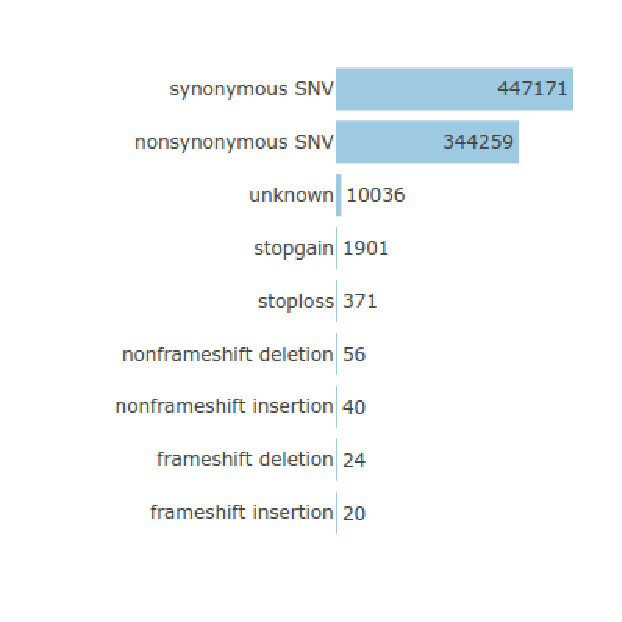
\includegraphics[width=0.35\textwidth]{Kap4/variantes.png}}
	\subfigure[Distribución de variantes por rango de edad]{
		\label{f:variantedad}
		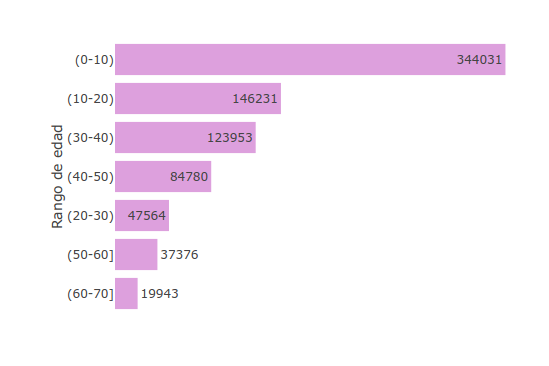
\includegraphics[width=0.55\textwidth]{Kap4/edad.png}}
	\caption{Distribución del tipo de variantes}
	\label{f:variantesgeneral}
\end{figure}

El estado alélico de las variantes (cigocidad) que se encuentran dentro de la base de datos se dividen en heterocigotas 458639 que corresponden al 57,05\% del total de las variantes  y homocigotas 345239 que corresponden al 42,95\%. La distribución de la cigocidad de las variantes se puede explicar desde el error que se puede generar en la identificación de las variantes dado que durante el llamado  de variantes es posible que una variante homocigota se catalogue como heterocigota, si durante el proceso de secuenciación se identifican erróneamente los nucleótidos \cite{Babraham2016}\cite{Pirooznia2014}. 

\section{Análisis textual de información clínica}

Las información clínica se encuentran en forma de documentos que contienen el diagnóstico de cada paciente al cual se realizó un procesamiento de lenguaje natural. El análisis de documentos corresponde a la agrupación de términos con el fin de encontrar grupos de pacientes con diagnósticos similares.
 
\subsection{Preprocesamiento.}
    
El proceso de limpieza y normalización de texto se realizo de la siguiente manera:

 \begin{enumerate}
 	\item Remoción de ``stop words'' en español, tildes y caracteres especiales como la letra ñ y todos los documentos se unificaron en letras minúsculas.
 	\item Creación de un diccionario de sinónimos, donde se reemplazaron palabras que hacen referencia a una misma característica, teniendo en cuenta la interpretación clínica. 
 	\item Cálculo de la frecuencias de palabras dentro de los documentos. 
 	\item Remoción de las palabras pam,pacientes, secuenciación y gen dado que no son un factor diferenciador de los documentos.  	  
 \end{enumerate}

\subsection{Análisis de frecuencia de palábras}

La figura \ref{fig:sin}(a) muestra las distribución de las palábras más frecuentes 30 palabras más frecuentes y \ref{fig:sin}(b) muestra una la nube de palabras teniendo en cuenta todos las palabras presentes en el diagnóstico.\\

\begin{figure}[H]
	\centering
	\subfigure[Nube de palabras]{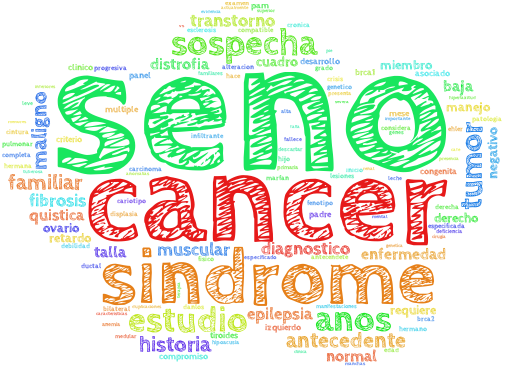
\includegraphics[width=60mm]{Kap4/sin_stop}}
	\subfigure[Frecuencia de términos]{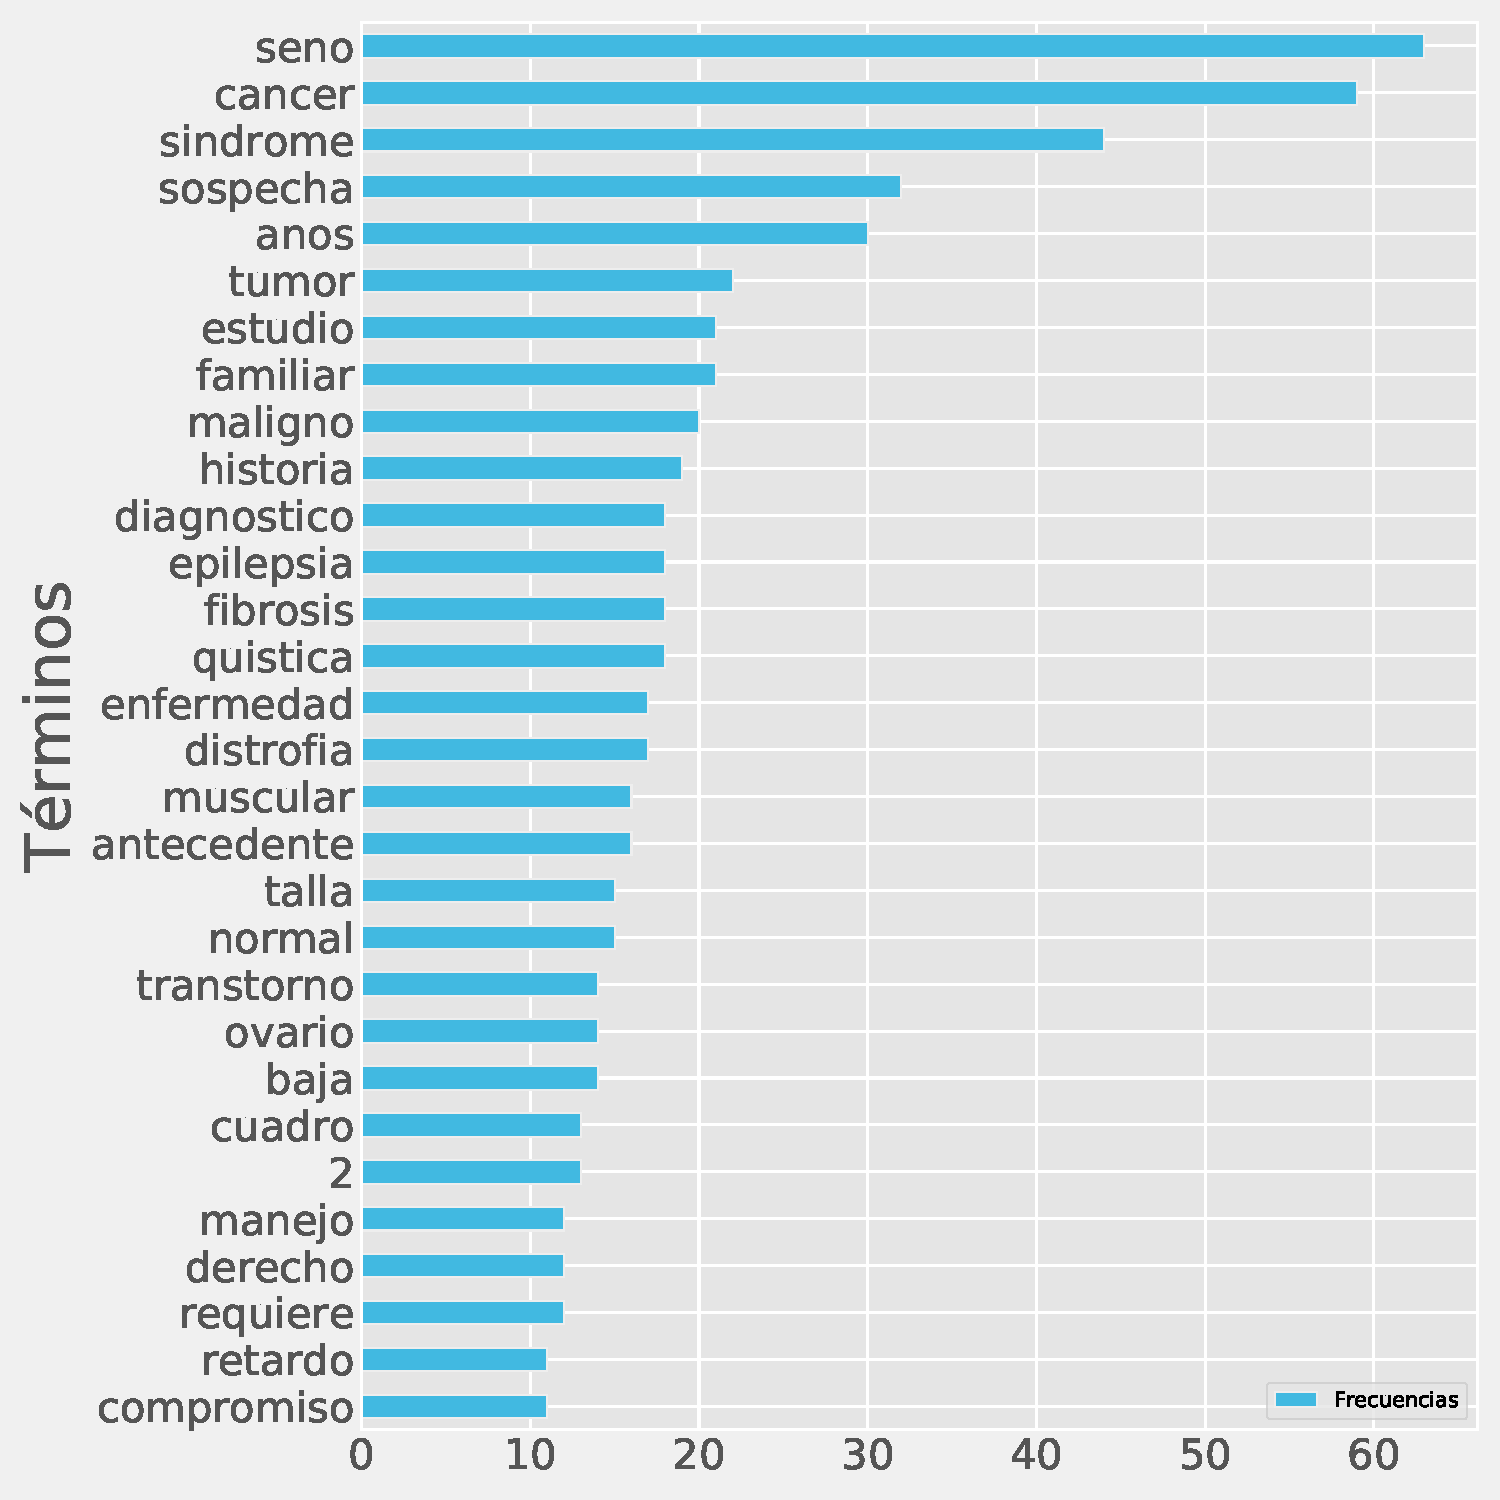
\includegraphics[width=60mm]{Kap4/frecuecias.pdf}}
	\caption{Palabras más frecuentes en el diagnóstico clínico  presentes en las historias clínicas } \label{fig:sin}
\end{figure} 

Las frecuencia de palabras muestran las principales características de la información clínica, siendo las palabras cáncer y seno los principales fenotipos, también se encuentra la palabra síndrome que puede asociarse a diferentes  enfermedades y la palabra sospecha hace referencia a diagnósticos ambiguos que pueden tener los pacientes, una de las contribuciones de la secuenciación es que basado en el fenotipo puede ayudar a un diagnóstico,entre diferentes síntomas y síndromes que pueden ser aplicados a enfermedades raras y complejas\cite{Tetreault2015a}.Sobre  la matriz  de frecuencias normalizada se cálculo la matriz tf-idf \\

La figura \ref{fig:IDFTF} representa la matriz IDF-TF de las 30 primeras palabras de los diagnósticos.  

\begin{figure}[H] 
	\centering
	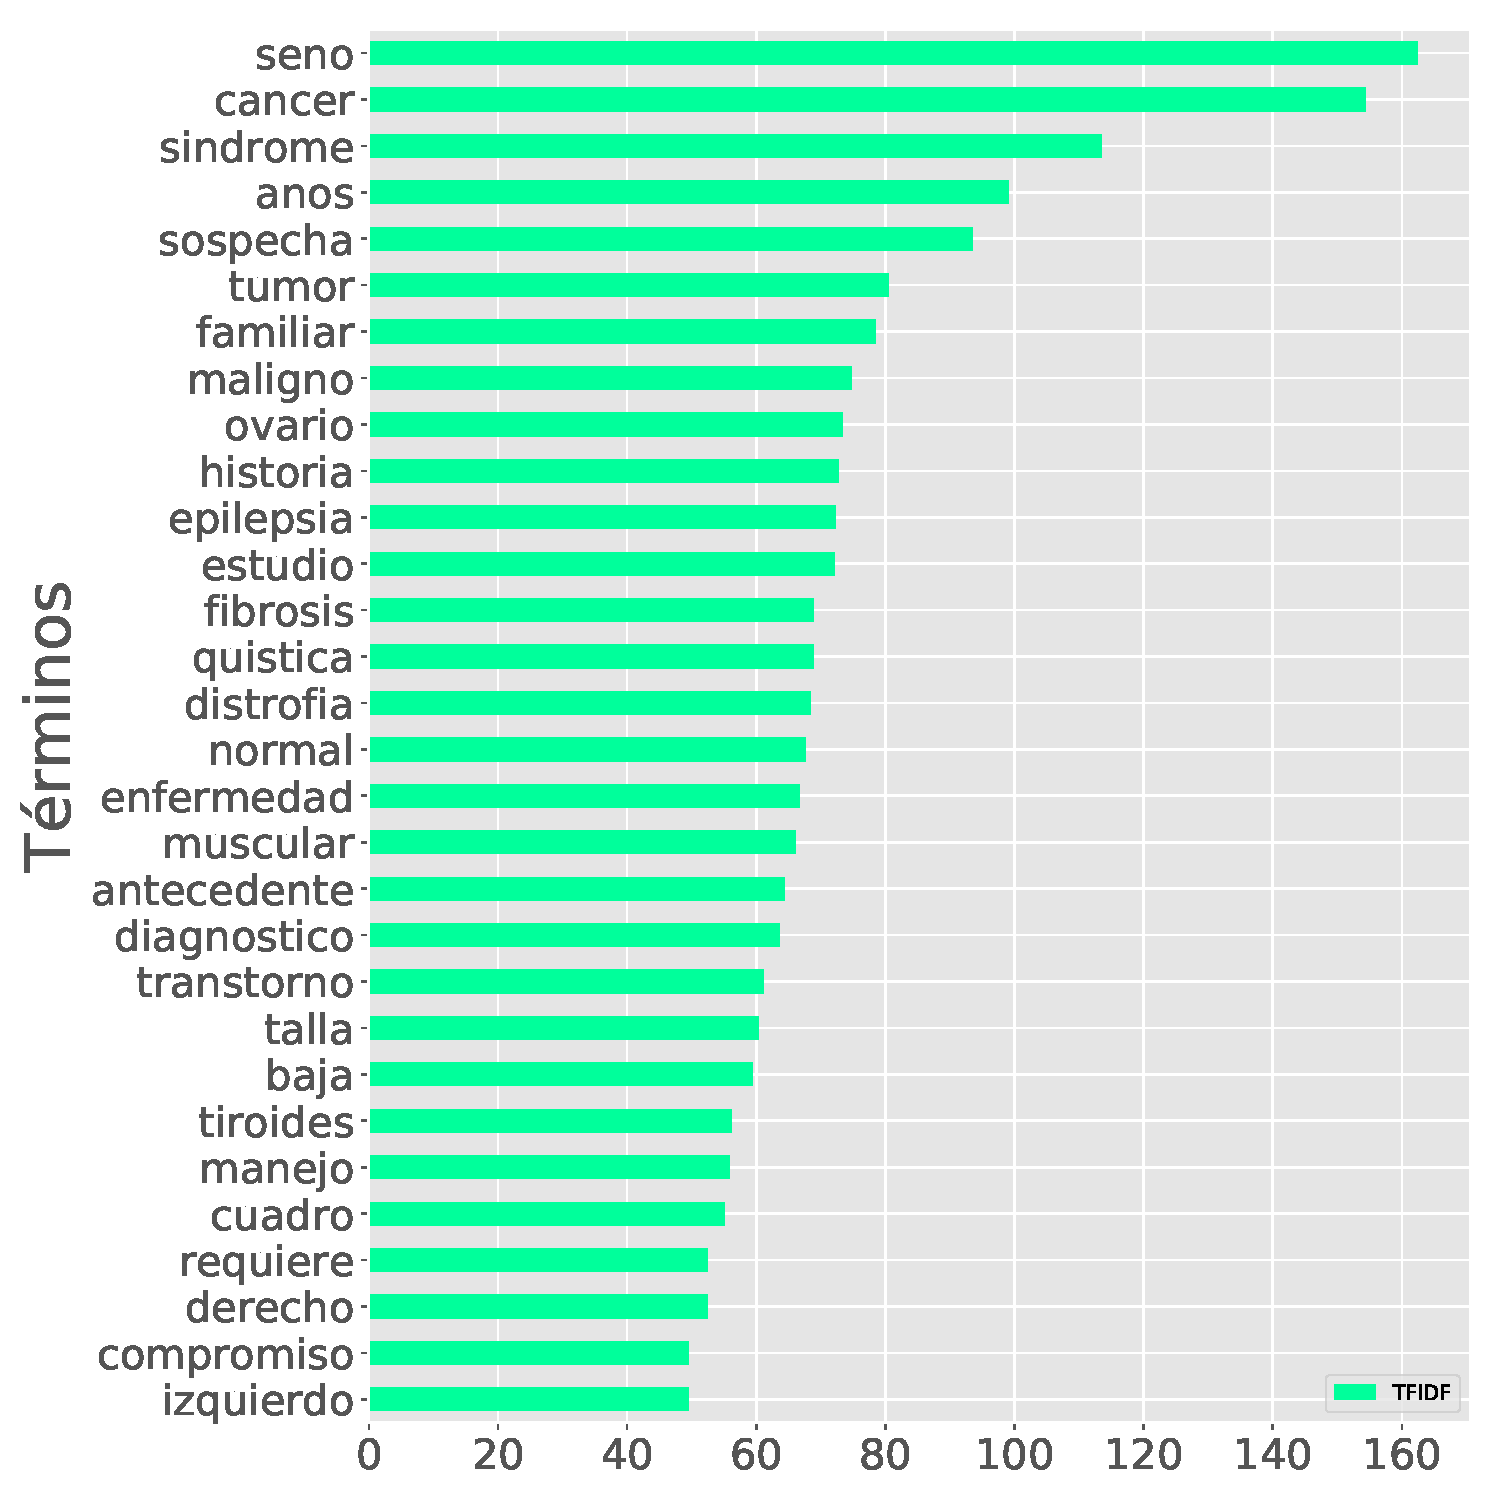
\includegraphics[width=0.5\textwidth]{Kap4/tfidf.pdf}
	\caption{TF-IDF} 
	\label{fig:IDFTF}
\end{figure}

Se calculo la similitud de coseno de acuerdo a la siguiente formula donde la similitud ente $u$  y $v$ está definida según la librería scipy de python \cite{scipy}:

$$   1 - \frac{u \cdot v}
{||u||_2 ||v||_2}. $$

donde $u.v$ donde el punto es el producto de $u$ y $v$.


\subsection{Caracterización de las historias clínicas usando diagnóstico}

Caracterizar las historias clínicas  de acuerdo al diagnóstico, permitirá entender grupos de diagnósticos similares y se podrán encontrar relaciones entre otras variedades que tengan un diagnóstico similar. Para esto se implemento un modelo de agrupamiento utilizando la matriz tf-idf y se aplicaron los algoritmos de k means y el algoritmo average  para identificar los grupos. Los pasos que se llevaron fueron:

\begin{enumerate}
	\item Estimación de el número de k optimo.
	\item Implementación del algortitmo average.
	\item Implementación del algoritmo k-means.
	\item Validación de los grupos.
	\item Análisis de resultados. 	  
\end{enumerate}


\subsection{Experimentación y validación del modelo de agrupamiento}

\subsubsection{Jerárquico}

A partir de la matriz tf-idf se cálculo la similaridad de coseno según recomendaciones \cite{Renganathan2017,Allahyari2017} y se aplico el el algoritmo average, la figura \ref{fig:jerarquico}} muestra el resultado:

\begin{figure}[H] 
	\centering
	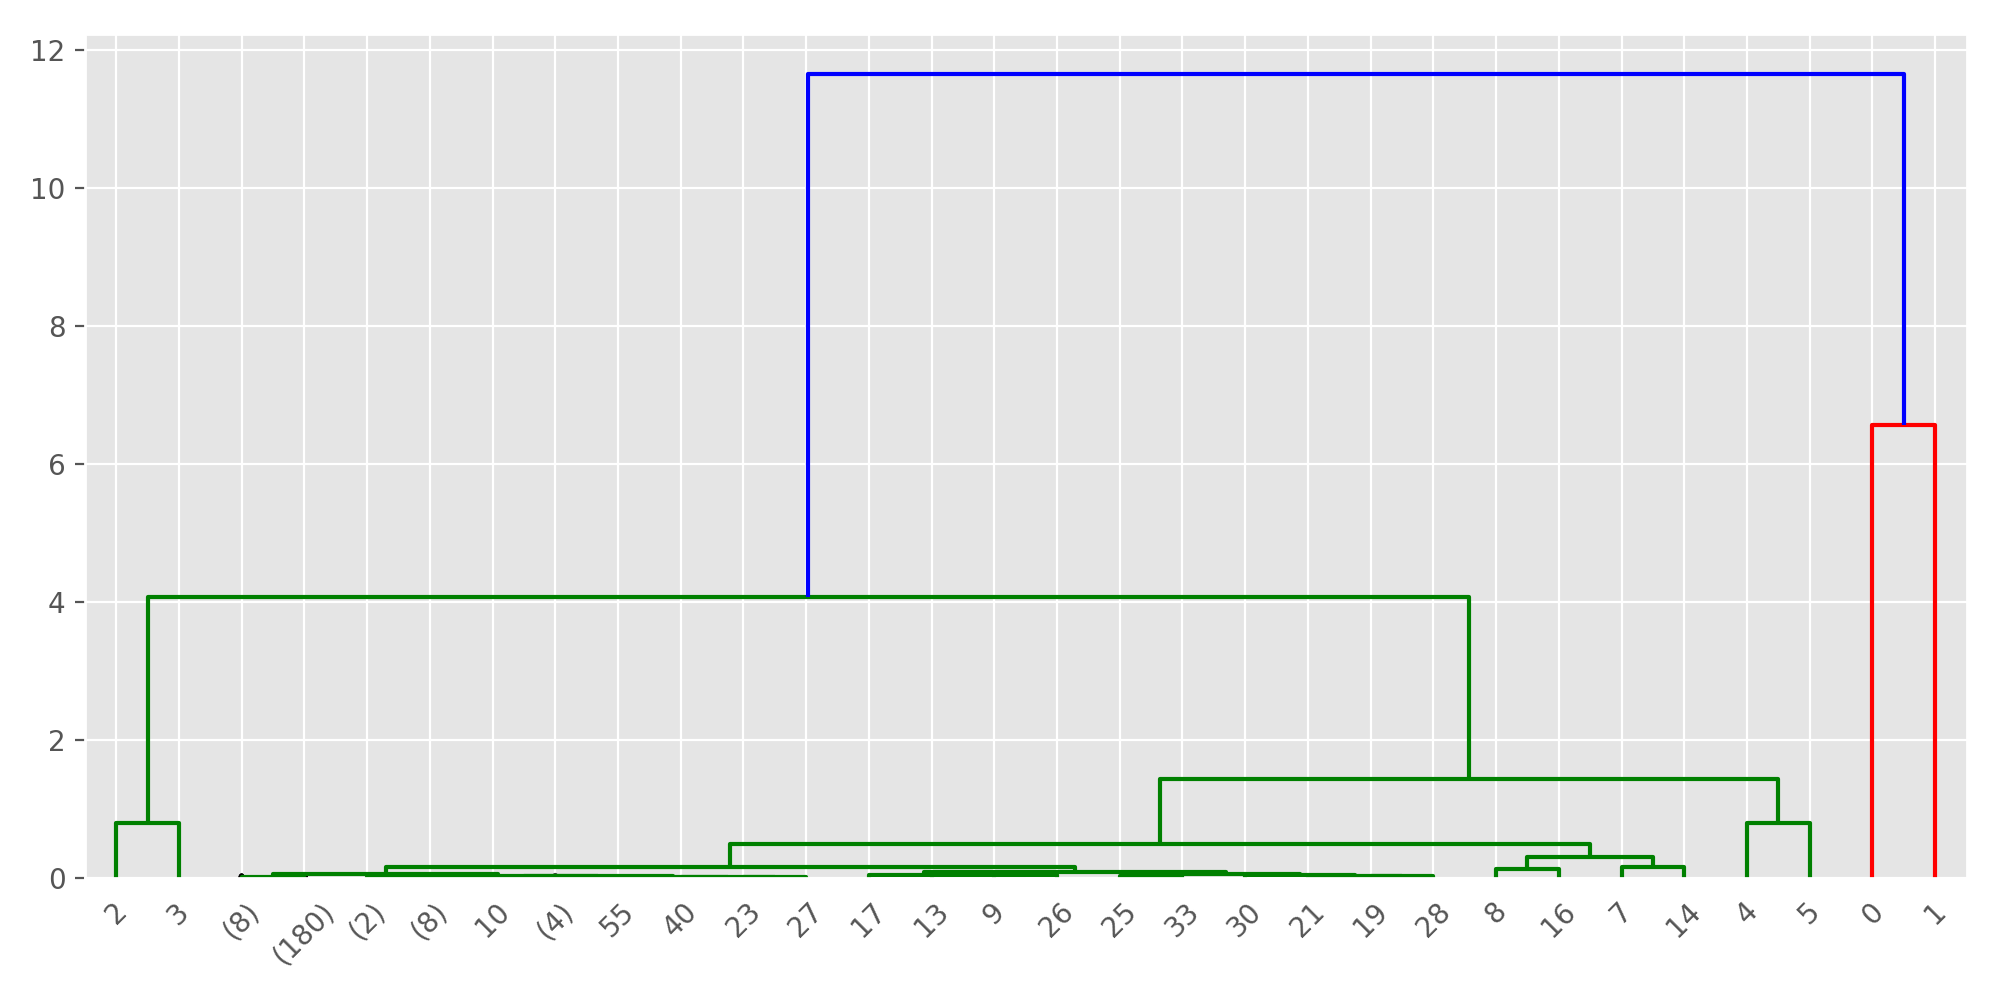
\includegraphics[width=0.8\textwidth]{Kap4/averagercortado}
	\caption{Grupos de diagnósticos} 
	\label{fig:jerarquico}
\end{figure}

La figura \ref{fig:jerarquico} muestra un resumen de como quedan agrupadas las historias clínicas, donde cada número representa el documento que corresponde al paciente, el documento cero pertenece al paciente uno, dado que para python el número inicial es cero. Se obtuvieron dos grupos, donde solo dos documentos quedaron agrupados dentro de un grupo, pero que al realizar la revisión son pacientes que no están relacionados en su diagnóstico,ya que el documento cero es de picos febriles (Síndrome febril) y el documento uno es de craneocitosis. El segundo grupo más grande se encuentran los demás documentos y se subdividen en nuevos grupos, que no se encuentran relacionados entre sí, pero comparten la palabra sospecha.\\

Para el presente trabajo esté agrupamiento de los diagnósticos no es optimo, pero muestra dos grandes grupos de diagnósticos. 

\subsubsection{k means}

El cálculo del error cuadrático vs el número de grupos se realizo utilizando la libreria de python scikit learn, donde se computa el valor de la inercia que es calculada como la suma de cuadrados por cada punto cercano al centroide y es asignado al grupo. Así que  $I = \sum_{i}(d(i,cr))$ donde $cr$ es el centroide que fue asignado al grupo y $d$ es la distancia cuadrada \cite{scikit-learn}. 

\begin{figure}[H]
	\centering
	\subfigure[Error cuadrático.]{
		\label{f:Clusters}
		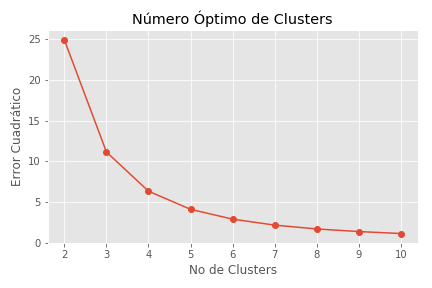
\includegraphics[width=0.35\textwidth]{Kap4/Clusters}}
	\subfigure[Valor Silhouette por cada grupo]{
		\label{f:S}
		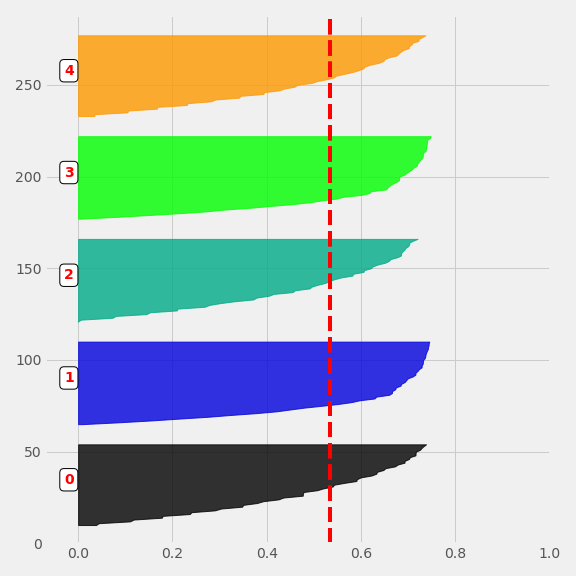
\includegraphics[width=0.35\textwidth]{Kap4/S}}
	\caption{Gráficos para la selección del número optimo de K}
	\label{f:medidas}
\end{figure}


Una vez se computo la inercia se realizo genero el gráfico del error cuadrático vs el número de grupos  la figura \ref{f:Clusters} muestra el gráfico de codo obtenido, donde se puede seleccionar el grupo 5 y 6 como óptimo de $K$. Para definir el número de optimo de $K$ también se computo el coeficiente de Silhouette  que fue de \textit{0.534}, adicionalmente se gráfico los valores de del coeficiente Silhouette para un $K$ = 5 y se presenta en la figura \ref{f:S}. \\

Los resultados de validación obtenidos fueron: homogeneidad 0.296, para integridad 1.0, para el V-measure 0.457. La homogeneidad perfecta sería con un valor de 1.0 pero lo obtenidos en los grupos fue una baja homogeneidad con una alta  integridad de 1.0 que muestra que las etiquetas son perfectamente completas,los grupos tienen  baja homogeneidad pero una alta integridad.\cite{scikit-learn}. 


\section{Asociación de grupos de historias clínicas con variantes}

Una vez realizado el agrupamiento de la información clínica se aplico un modelo de asociación de las variantes con los grupos obtenidos de la siguiente forma:

\begin{enumerate}
	\item Consulta de las variantes que se encontraban en cada grupo.
	\item Asociación de las variantes por grupo.
	\item Asociación de las variantes por toda la información de la base de datos filtrada por el gen CFTR como caso de ejemplo.
\end{enumerate}

\subsection{Variantes vistas como transacciones}

Uno de los criterios más importantes para la clasificación de variantes es la frecuencia con la que se presentan las variantes dentro de una población, según la asociación americana de genética médica \cite{Laboratories2015}, adicionalmente uno de los retos del análisis de variantes es el estado alélico de las mismas; existen tres tipos de estado alélico: el primero es el homocigoto donde los dos alélos son idénticos, el heterocigoto cuando los alélos son diferentes y el heterocigoto compuesto que hace referencia a dos variantes heterocigotas que afectan diferentes regiones del mismo gen o de genes distintos pero que cumplen una misma función biologíca \cite{Klug2013,Compound2012}.\\

Teniendo en cuenta lo anterior es importante visualizar el estado alélico de las variantes \cite{Hannah-Shmouni2015,Laboratories2015} ya que pueden tener un impacto el fenotipo del paciente.La identificación entre la relación genotipo-fenotipo, se ingresan como frecuencia de variación, que para el trabajo caso serían las transacciones\cite{Breuer2017}.\\

La relación genotipo-fenotipo que se observa es  la de utilizar los datos de gen, el tipo de variante, la edad, el género y el clúster (representación del fenotipo), como los patrones a recibir, para mirar las asociaciones y las reglas dentro de todo el set de datos. La identificación de patrones frecuentes, puede ser aprovechado por reglas de asociación y con ello identificar los estados alélicos de las variantes en los genes que se encuentran dentro de la base de datos \cite{breuler2017}.\\

Para el presente trabajo los items son id del paciente, gen, cigocidad(estado alélico de las variantes), tipo de variante, rango de edad, genero y grupo al que pertenece el paciente, mientras que las transacciones son las variantes a las cuales se les asigna un ID iniciando con el número 1.

\begin{table}[H]
	\centering
	\resizebox{16cm}{!}{
	\begin{tabular}{ll|l|l|l|l|l|l|}
		\cline{3-8}
		&   & \textbf{Items} & Tipo de variante & Cigocidad & Rango de edad & Genero & Grupo \\ \hline
		\multicolumn{1}{|l|}{\multirow{2}{*}{\textbf{Transacciones}}} & 1 & BRCA1          & No sinónima      & Het       & (30-40)       & F      & C1      \\ \cline{2-8} 
		\multicolumn{1}{|l|}{}                                        & 2 & RB1            & Stop gain        & Het       & (0-10)        & F      & C5      \\ \hline
	\end{tabular}
}
\caption{ Tabla de items y transacciones}
\label{tabla:items}
\end{table}
 
La tabla \ref{tabla:items} muestra los items utilizados para ser asociados, y las transacciones que son los los ID por cada conjunto de items que se encuentran dentro de la base de datos.

\subsection{Experimentos}

La confianza y el soporte para este trabajo se ajusto a partir de los resultados experimentales, donde se observo que el soporte es inversamente proporcional a la confianza, esto se debe a la cantidad de variantes que se encuentran dentro de la base de datos. Al correr un experimento con un soporte mínimo de 0.2 y una confianza mínima de 0.9 no se obtuvo ningún tipo de regla, por lo tanto, estos valores se fueron ajustando disminuyendo en 0.1 el valor de la confianza y el soporte.\\

Finalmente se ajusto un soporte de 0.05 y una confianza de 0.5, dado que con un soporte de 0.1 solo se generaban 5 reglas, utilizando toda los datos disponibles. Una vez realizado este ajuste se dejaron los valores de soporte y confianza igual para todos los experimentos, también se realizo la remoción de reglas redundantes.\\

Una vez se ajustaron los valores de soporte y confianza se realizaron 12 experimentos, los primeros 5 experimentos con todas las variante dentro del set de datos junto a su grupos, otro a todo el conjunto de datos aplicado con los datos y filtrado por el gen CFTR. Se volvieron a repetir los mismos experimentos pero removiendo las variantes sinónimas que son las más frecuentes dentro del conjunto de datos.


\subsection{Resultados} 

Teniendo en cuenta las medidas de validación encontramos  5 grupos con las siguientes estructuras:

\begin{figure}[H]
	\centering
	\subfigure[Nube de palabras]{\label{f:nube1}
		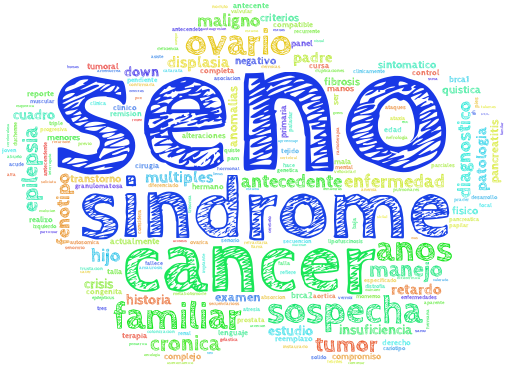
\includegraphics[width=70mm]{Kap4/cluster1}}
	\subfigure[Distribucón demográfica de los pacientes]{\label{fig:grupo1}
		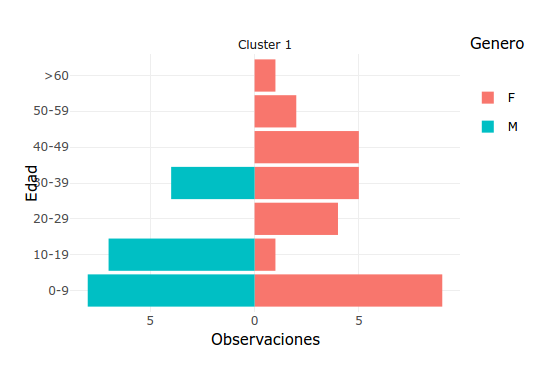
\includegraphics[width=70mm]{Kap4/edadc1}}
	\caption{Grupo 1}
	\label{f:grupo11}
\end{figure} 


La figura \ref{f:grupo11} representa el grupo 1 con la frecuencia de palabras que se agrupadas y la figura \ref{f:nube1}  se muestra la frecuencia de palabras, siendo seno,síndrome y cáncer son las palabras más frecuentes, junto con ovario,familiar sospecha y epilepsia. La figura \ref{fig:grupo1} representa la distribución de pacientes por edad y genero dentro del grupo por rango de edad en un intervalo de 10 años.\\

\begin{figure}[H]
	\centering
	\subfigure[Reglas de asociacióncon variantes sinónimas.]{\label{fig:re1}
		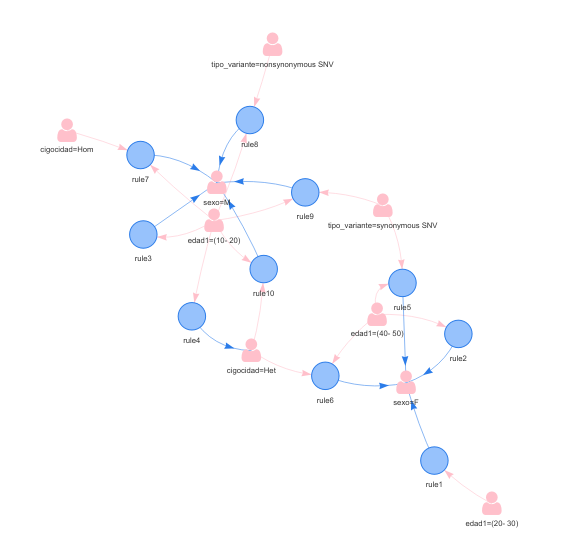
\includegraphics[width=100mm]{Kap4/reglas1_1}}
	\subfigure[Reglas de asociación sin variantes sinónimas]{\label{fig:r1}
		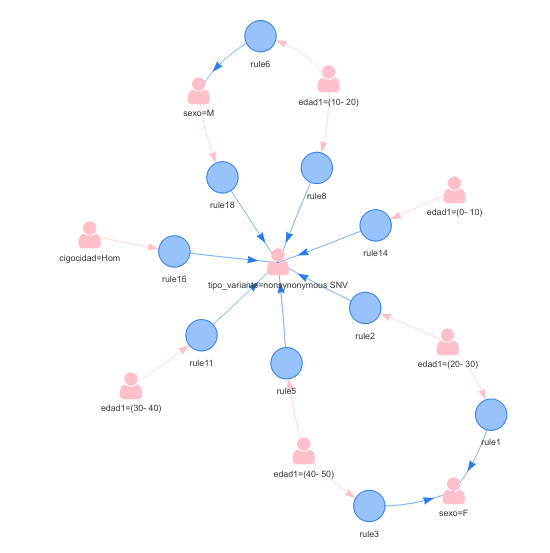
\includegraphics[width=100mm]{Kap4/reglas1_2}}
	\caption{Reglas de asociación del grupo 1.}
	\label{fig:reglas1}
\end{figure}

La figura \ref{fig:reglas1} que muestra la asociación de variantes con información clínica del grupo 1.En la figura \label{fig:re1} se presentan los resultados reglas de asociación sin remover las variantes sinónimas. Para el presente grupo se obtuvo dos tipos de variantes  distribuidas por género, donde el masculino presenta variantes  sinónimas y que son pacientes con un rango de edad entre 10 y 20 años, con un estado alélico homocigoto, para este grupo se observa una alta diferencia en las reglas ambos géneros, donde las pacientes de género femenino tienen variantes sinónimas con estado heterocigotas y con mayor diferencia de rango  de edad, pero las pacientes con la edad de 10 a 20 años no presentan variantes homocigotas a diferencia de los pacientes de genero masculino. \\

En cuanto a las reglas removiendo las variantes sinónimas que se muestran en la figura  \ref{fig:r1}, se observa que  nuevamente la distribución que los pacientes masculinos son pacientes entre 10 y 20 años, con variantes heterocigotas , mientras que para el genero femenino se tienen rangos de edad más amplios desde la edad  de 0 a 50 años, en este caso las variantes homocigotas están como una regla independiente.

\subsubsection*{Grupo 2}

\begin{figure}[H]
	\centering
	\subfigure[Nube de palabras]{\label{fig:nube2}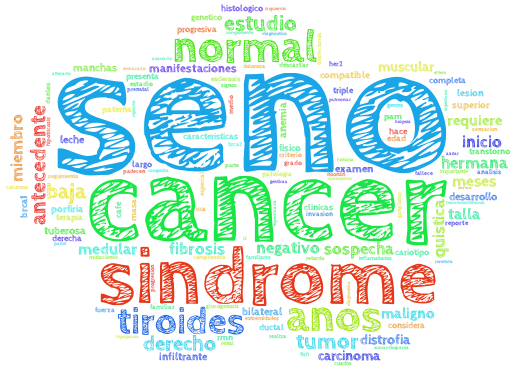
\includegraphics[width=60mm]{Kap4/cluster2}}
	\subfigure[Rango de edad en décadas.]{\label{fig:demo2}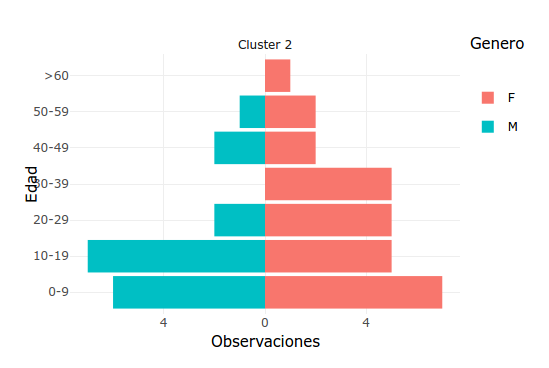
\includegraphics[width=60mm]{Kap4/edadc2}}
	\caption{Grupo 2} \label{fig:c2}
\end{figure}

En la figura \ref{fig:nube2} se observa que al igual que el grupo 1 las palabras más frecuentes son cáncer,seno y síndrome, pero aparecen palabras como antecedente tiroides y hermana,según la \ref{fig:demo2} se observa rangos de edad entre 20 y 30 años y para el rango entre 30 y 40 años y para mayores de 60 no hay pacientes masculinos, siendo este un grupo representado principalmente por pacientes femeninas.  

\begin{figure}[H]
	\centering
	\subfigure[Reglas de asociación con variantes sinonimas]{\label{fig:reglas2.1}
		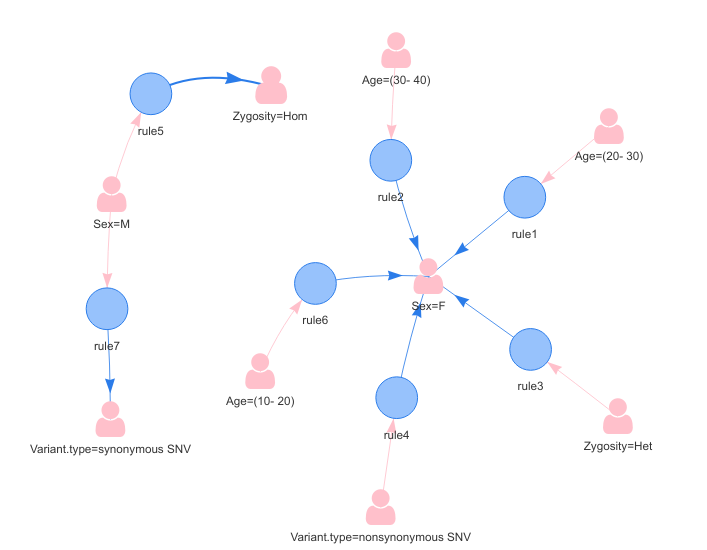
\includegraphics[width=120mm]{Kap4/reglas2_1}}
	\subfigure[Reglas de asociación sin variantes sinonimas]{\label{fig:reglas2_2}
		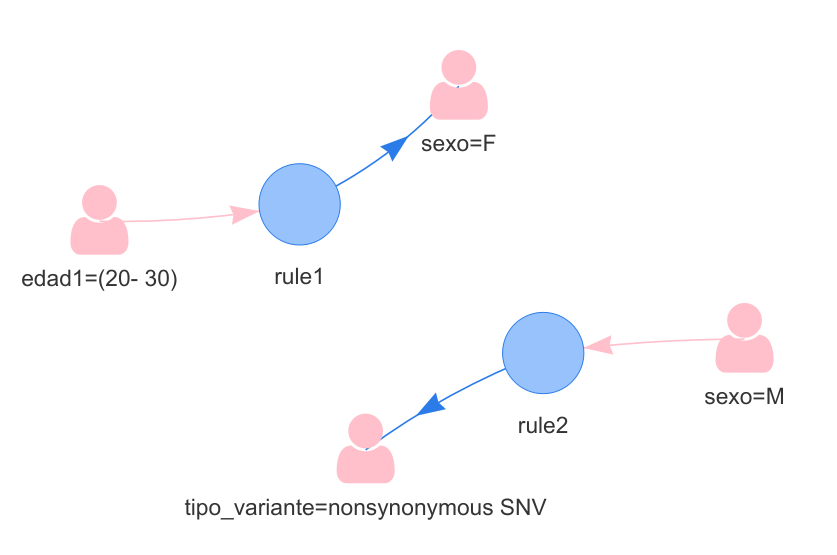
\includegraphics[width=120mm]{Kap4/reglas2_2}}
	\caption{Reglas de asociación del grupo 2}\label{fig:reglas2}
\end{figure}

La figura \ref{fig:reglas2.1} nos muestran asociación de variantes al género femenino con tres rangos de edad distinto y con el estados alélicos heterocigoto mientras que para el género masculino se presentan variantes homocigotas,mientras que al remover las variantes sinónimas en la figura \ref{fig:reglas2_2} solo queda un rango de edad para el género femenino asociado unicamente a un rango de edad y una regla para el genero másculino asociado unicamente al tipo de variante.En este grupo se observan dos reglas no relacionadas para cada género.

\subsubsection*{Grupo 3}

\begin{figure}[h]
	\centering
	\subfigure[Nube de palabras.]{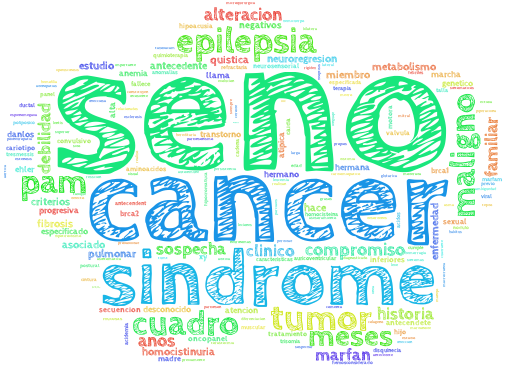
\includegraphics[width=60mm]{Kap4/cluster3}}
	\subfigure[Rango de edad en décadas.]{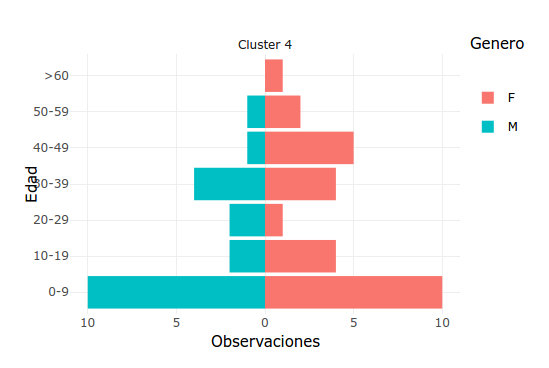
\includegraphics[width=60mm]{Kap4/edadc3}}
	\caption{Grupo 3} \label{fig:c3}
\end{figure}

La figura \ref{fig:c3}(a) nos muestra la frecuencia de palabras donde seno, cáncer y síndrome se tiene la palabra pam tumor maligno y epilepsia. La figura \ref{fig:c3}(b) muestra la distribución donde no hay pacientes de genero masculino para mayores de 60 años.  

\begin{figure}[H]
	\centering
	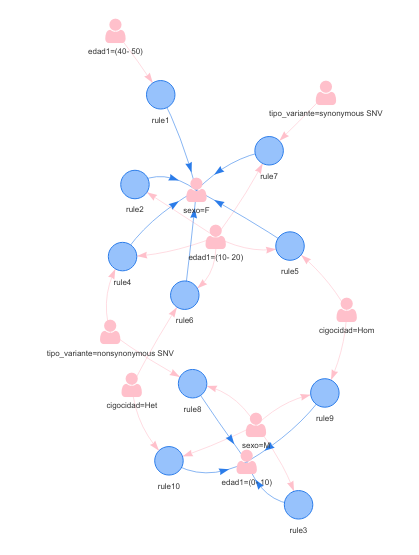
\includegraphics[width=0.8\textwidth]{Kap4/reglas3_1}
	\caption{Reglas de asociación del grupo 3 con variantes sinónimas.} \label{fig:r3}
\end{figure}

La figura \ref{fig:r3} muestra las asociaciones entre las variantes sinónimas al género femenino, donde las variantes sinónimas se encuentran en mayor frecuencia a el rango de edad entre 40 a 50 años y son heterocigotas, se presenta una frecuencia de pacientes entre los 10 y 20 años a variantes con un estado alélico homocigoto y al genero femenino, mientras que para el rango de edad de 0 a 10 años el estado alélico esta dividido entre homocigoto y heterocigoto, pero con variantes no sinónimas.

\begin{figure}[H]
	\centering
	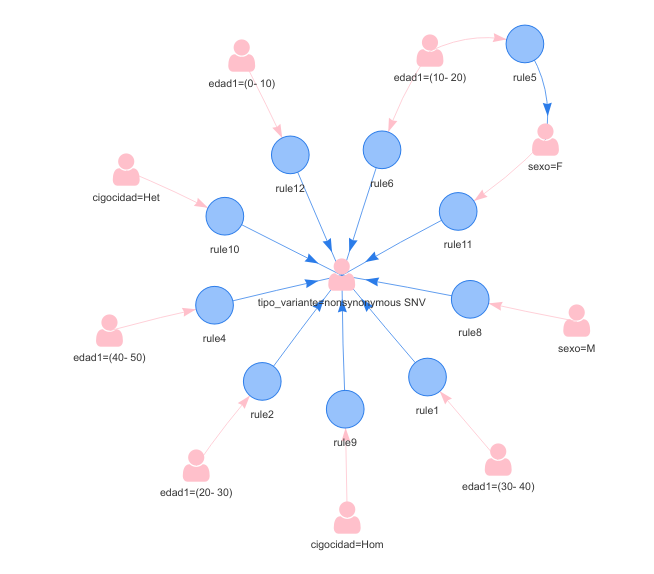
\includegraphics[width=0.8\textwidth]{Kap4/reglas3_2}
	\caption{Reglas de asociación del grupo 3 sin variantes sinónimas.} \label{fig:re3}
\end{figure}

La figura \ref{fig:re3} muestra la asociación de rangos de edades con las variantes no sinónimas donde las variantes del género masculino son para un rango de edad entre 0 y 10 años de edad, mientras que los demás rangos pertenecen no está asociados a un género en especifico, para el genero femenino se observa que el rango de edad es de 10 a 20 y de 40 a 50,mientras que los demás rangos de edad no muestran otro tipo de asociación para este tipo de variantes.  

\subsubsection*{Grupo 4}
\begin{figure}[H]
	\centering
	\subfigure[Nube de palabras]{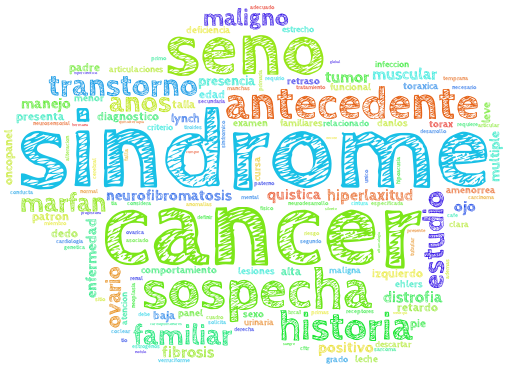
\includegraphics[width=60mm]{Kap4/cluster4}}
	\subfigure[Rango de edad en decadas]{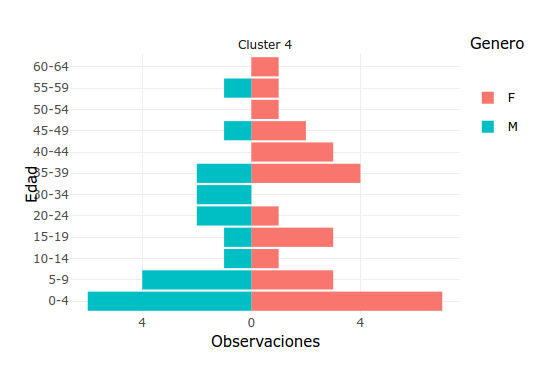
\includegraphics[width=60mm]{Kap4/edadc4}}
	\caption{Grupo 4} \label{fig:c4}
\end{figure}

La figura \ref{fig:c4}(a) muestra las frecuencias de palabras que son síndrome y cáncer, pero la palabra seno no es tan predominante como los grupos anteriores, se tienen otras palabras como sospecha, antecedente, historia y trastorno. La figura \ref{fig:c4}(b) muestra que la para este grupo los rangos de edad de 40 a 45 años, de 50 a 55 años y mayores de 60 no cuentan con representación de pacientes de género femenino.

\begin{figure}[H]
	\centering
	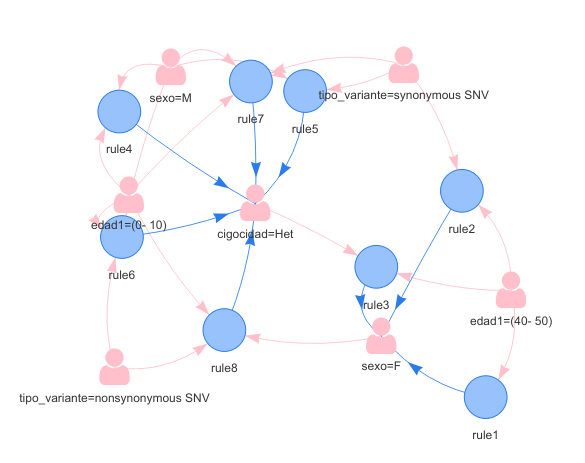
\includegraphics[width=0.8\textwidth]{Kap4/reglas4_1}
	\caption{Reglas de asociación del grupo 4 con variantes sinónimas.} \label{fig:r4}
\end{figure}

La figura \ref{fig:r4} muestra la asociación de las variante heterocigotas a pacientes masculinos de tipo no sinónimas con un rango de edad de 0 a 10 años, mientras que las variantes sinónimas se asocian a pacientes con un rango de edad de 40 a 50 años y son pacientes femeninas. 

\begin{figure}[H]
	\centering
	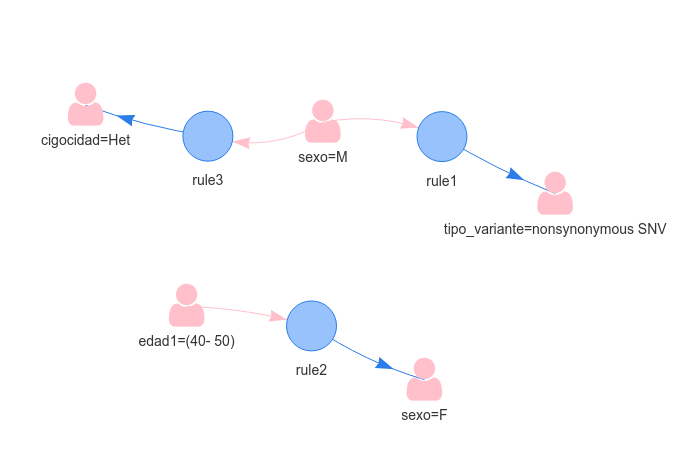
\includegraphics[width=0.8\textwidth]{Kap4/reglas4_2}
	\caption{Reglas de asociación del grupo 4 sin variantes sinónimas.} \label{fig:re4}
\end{figure}

La figura \ref{fig:re4} muestra reglas  donde las reglas del grupo nuevamente se discrimina que las variantes no sinónimas son femeninas y están en un rango de edad de (40-50), mientras que las variantes heterocigotas se encuentran en un rango de edad de 0 a 10 años. 

\subsubsection*{Grupo 5}

\begin{figure}[H]
	\centering
	\subfigure[Nube de palabras]{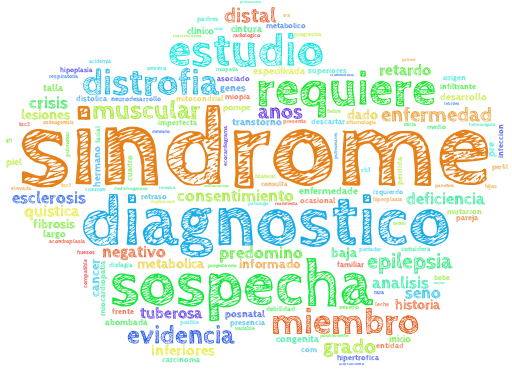
\includegraphics[width=60mm]{Kap4/cluster5}}
	\subfigure[Rango de edad en décadas]{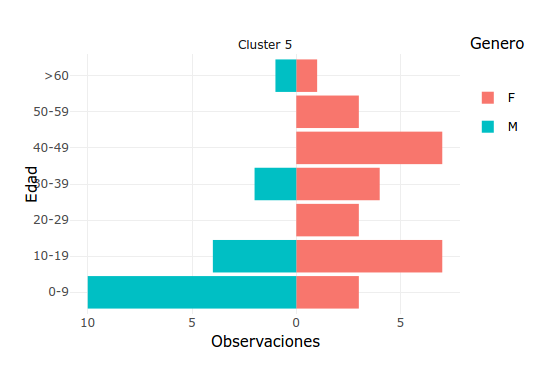
\includegraphics[width=60mm]{Kap4/edadc5}}
	\caption{Grupo 5} \label{fig:c5}
\end{figure}

La figura \ref{fig:c5}(a) presenta la frecuencia de palabras y este grupo a diferencia de todos los anteriores no presenta la palabras cáncer y seno, como las más frecuentes pero si presenta con más alta frecuencia son síndrome, diagnóstico, estudio, distrofia, requiere y miembro. La figura \ref{fig:c5}(b) muestra la distribución de pacientes por edad y género donde los rangos de 20 a 30 y 40 a 60 no se encuentran pacientes de género masculino, aunque tiene 10 pacientes masculinos en el rango de edad de 0 a 10 años.

\begin{figure}[H]
	\centering
	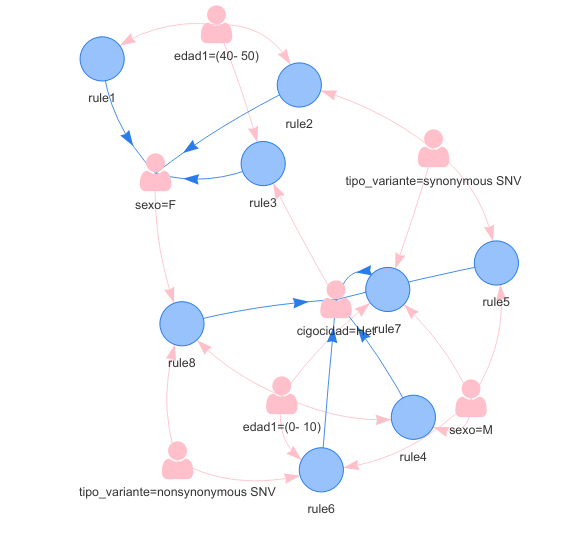
\includegraphics[width=0.8\textwidth]{Kap4/reglas5_1}
	\caption{Reglas de asociación del grupo 5 con variantes sinónimas} \label{fig:r5}
\end{figure}

La figura \ref{fig:r5} muestra la asociación de las variantes al genero femenino con un rango de edad de 40 a 50 años y de tipo sinónimas, mientras que las de género masculino  a un rango de edad de 0 a 10 años con variantes no sinónimas.

\begin{figure}[H]
	\centering
	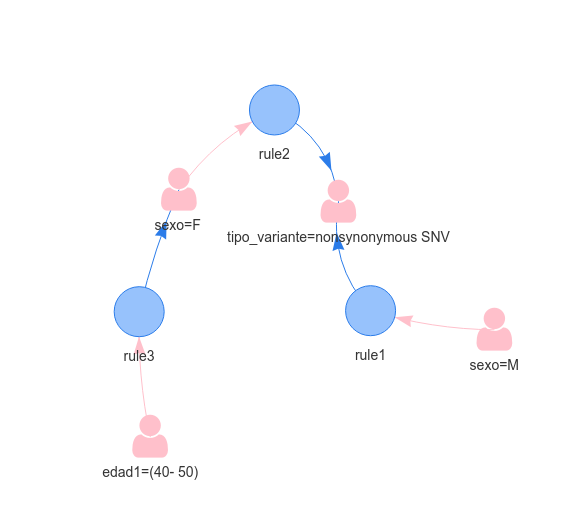
\includegraphics[width=0.7\textwidth]{Kap4/reglas5_2}
	\caption{Reglas de asociación del grupo 5 sin variantes sinónimas} \label{fig:re5}
\end{figure}

La figura \ref{fig:re5} presenta que las variante no sinónimas son más frecuentes en los pacientes con un rando de edad de 0 a 10 años y que las variantes no sinónimas presentan la regla que las variantes se encuentran en un rango de 0 a 50 años de edad son de pacientes femeninas. 


\subsubsection*{CFTR}

Visualización de reglas de asociación para toda la base de datos utilizando el gen CFTR como filtro. 

\begin{figure}[H]
	\centering
	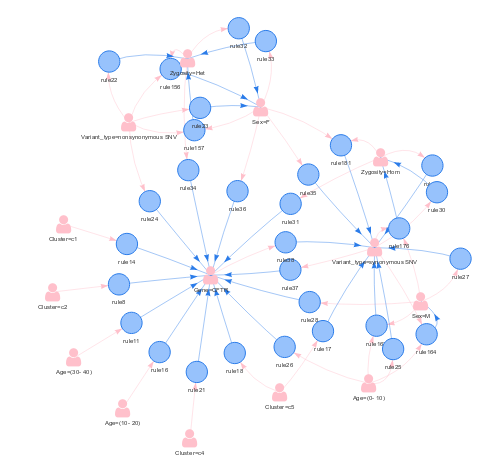
\includegraphics[width=0.87\textwidth]{Kap4/CFTR1}
	\caption{Reglas de asociación con variantes sinónimas} \label{fig:r6}
\end{figure}

La figura \ref{fig:r6} muestra las reglas 30 primeras reglas filtradas por el soporte con para toda la base de datos utilizando parámetro el gen CFTR, donde se observa que las variantes homocigotas son de tipo sinónimas y están más representadas en pacientes de ambos géneros, también se denota una frecuencia en pacientes que tienen entre 0 y 10 años de edad con variantes en este gen son de género masculino. \\

Las pacientes femeninas se tiene el caso de que las variantes son no sinonimas y no hay un  rango de edad directamente asociado a las pacientes femeninas. Los rangos de edad de 10 a 20 y de 30 a 40 tienen una frecuencia de variantes para el gen CFTR igual o mayor al 60\%, lo mismo se presenta con grupo 1,2 y 4. Para grupo 5 si se presenta una alta frecuencia de variantes sinónimas, mientras que para el grupo 3 no aparecen reglas con alta frecuencia con variantes en el gen CFTR. 

\begin{figure}[H]
	\centering
	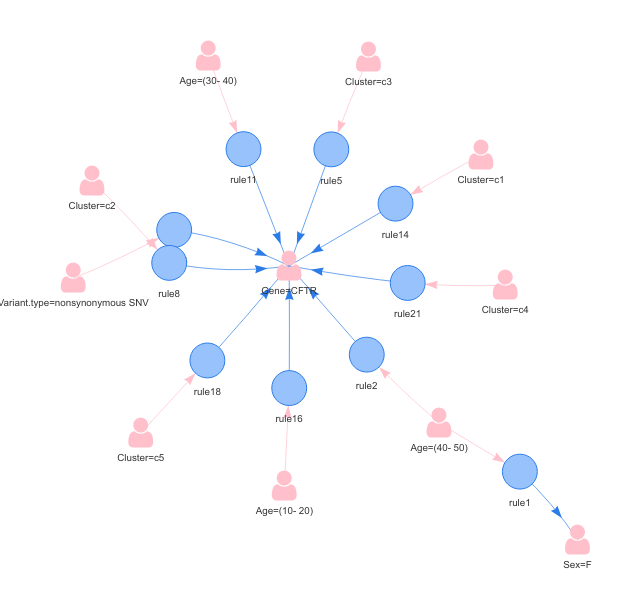
\includegraphics[width=0.8\textwidth]{Kap4/CFTR2}
	\caption{Reglas de asociación sin variantes sinónimas} \label{fig:re6}
\end{figure}

La figura \ref{fig:re6} muestra que el estado alélico de las variantes que no son sinónimas, y el estado alélico es heterocigoto para ambos generos, pero el rango de edad entre 0 y 10 años es frecuente para este tipo de variantes,a diferencia de la figura \label{fig:r6} solo se observa una alta frecuencia de las variantes no sinónimas al gen CFTR en grupo 4.  

\section{Prototipo de visualización}

Finalmente se desarrollo un dashboard utilizando la herramienta R, para mostrar todos los resultados obtenidas en el presente trabajo, para que las variantes que fueron encontradas puedan ser consultadas por la comunidad académica y científica. Este aplicativo presenta una pestaña general que muestra, la distribución demográfica de la población, la distribución del tipo de variantes encontradas y la distribución de las variantes encontradas por rangos de edad. Posteriormente se muestra una pestaña con cada grupo, donde se muestran las reglas de asociación obtenidas, la frecuencia de palabras del grupo y los rangos de edad por genero del grupo. Finalmente se muestra las reglas de asociación para el gen CFTR sin las variantes sinónimas y una tabla final con las variantes anotadas se obtuvieron. La figura \ref{fig:dash} muestra un screenshot  del aplicativo de visualización desarrollado, en la que se muestra los análisis exploratorios de las variantes.

\begin{figure}[H]
	\centering
	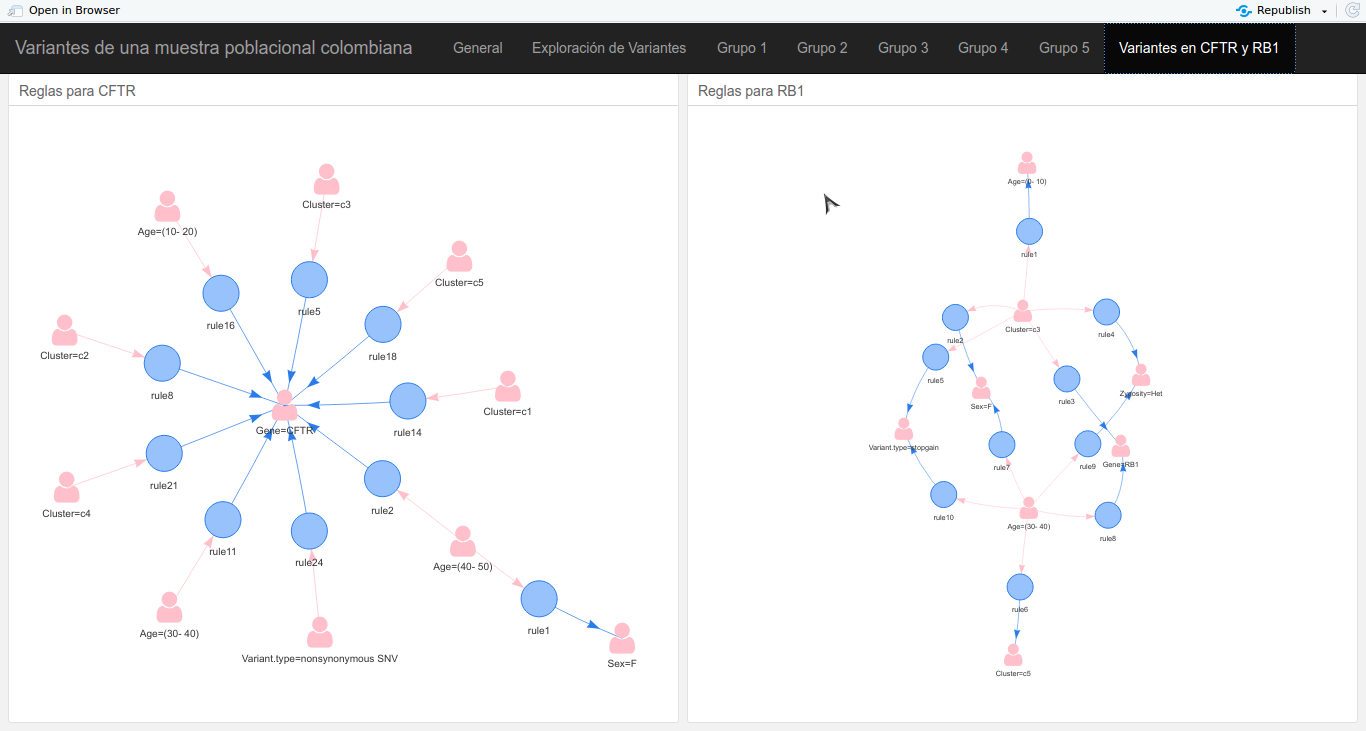
\includegraphics[width=1\textwidth]{Kap4/dash}
	\caption{Screenshot del dashboard desarrollado} \label{fig:dash}
\end{figure}

\section{Discusión}

El presente trabajo presenta los resultados de las variantes de la muestra poblacional que es de 227 pacientes y se cuenta con información como edad y genero,además que son pertenecientes a diferentes regiones del país (las muestras fueron remitidas de diferentes instituciones a nivel nacional, las muestras no contaban con la ubicación geográfica del paciente), esto en comparación con el proyecto de 1000 genomas, donde se secuenciaron 136 individuos de la ciudad de Medellín-Antioquia y el cual es un set de datos que no representan la población colombiana que es altamente diversa \cite{GabrielBedoya,Consortium2012}. Los datos que se encuentran dentro de este proyecto son utilizados principalmente para realizar análisis de ancestria \cite{Rishishwar2015a} y no evaluación de variantes dentro de la población, que igualmente no reflejan la ancestria y mezcla de la población colombiana. 

\subsection{Asociación de variantes con sus grupos de características clínicas.}

Los resultados de los grupos reflejan las características clínicas que se encuentran dentro de la base de datos, siendo el cáncer de seno el principal casual para llevar acabo las pruebas de secuenciación, esto corresponde con una de las bases para realizar la prueba de secuenciación en Colombia, ya que su valor diagnóstico y pronostico ha sido ampliamente estudiado en el país donde se da la importancia de la evaluación de la frecuencia de variantes en los genes BRCA1 y BRCA2 dentro de nuestra población, esto explica la razón de la alta frecuencia de las palabras cáncer y seno en cuatro de los cinco grupos obtenidos \cite{Ignacio2017,Arias-blanco2015}.\\

Los pacientes que se encuentran entre 0 y 10 años son la población más alta dentro de la base de datos (96 individuos)  y los que más variantes tienen, a pesar de ello las variantes que se presentan en este grupo poblacional no presentan la mismas reglas de asociación en los grupos frecuencia por ejemplo en el grupo 2 con las variantes \ref{fig:reglas2_1} se observa que no hay reglas frecuentes.\\ 

Los 4 primeros grupos están siendo representados por palabras similares, en el cuarto grupo la frecuencia de la palabra seno disminuye en comparación con los otros tres, se muestran diferencias significativas entre los rangos de edad y la distribución de géneros en cada uno de los grupos, y al incluir las reglas de asociación de cada uno de los grupos se tiene que las variantes no son iguales, inclusive a pesar de que la representación de pacientes femeninas aún es más alta la distribución de sus variantes difiere entre grupos, a pesar de que la homogeneidad de los mismos es baja, la diferencia entre cluters la composición de variantes y pacientes es altamente notoria.\\  

El grupo 5 que es único grupo las palabras cáncer y seno como las palabras más frecuentes, pero si la palabra síndrome que es común en todos los clústers, al hacer una evaluación de los pacientes, en este grupo se tienen otras palabras por lo tanto son pacientes que vienen por otras causas distintas a cáncer de seno, también es un grupo con una representación más alta de hombres. Este grupo atípico tiene una regla donde se muestra que las variantes heterocigotas no sinonimas se encuentran  en pacientes de 0 a 10 años. El hecho de que este grupo no asocie su variantes a un genero y si a un estado alélico nos puede llegar a mostrar que este grupo de pacientes tienen variantes autosomicas dominantes o variantes heterocigotas compuestas, y que las manifestaciones clínicas se presentan en una edad temprana \cite{Kamphans2013}. \\

La identificación de las causas genéticas de enfermedades por medio de la priorización de variantes partiendo de su tipo, deja una pobre aplicación de las variantes que causan perdida de la función biológica dependiendo de su estado alélico \cite{Eilbeck2017} dado que en las bases de datos normalmente el estado alélico no está disponible y su interpretación puede ser compleja \cite{Stenson2017} en el presente trabajo se muestra las variantes y su estado alélico dentro de la población muestreada. 


\subsection{Variantes con el gen CFTR}

Las variantes del gen CFTR son asociadas a la fibrosis quistica, ya que pueden ser causantes de perdida de la función biologica de la proteína, aunque la relación de las variantes con las manifestaciones no está completamente identificada, una de las razones por lo que su relación entre variante y enfermedad esta dada por la complejidad alélica de las variantes. Para este gen en particular se han reportado más de 2000 variantes pero solo unas pocas son asociadas a fibrosis quistica aproximadamente el 10\% han sido asociadas a variantes y su estado alélico. Se ha estimado que las técnicas de NGS es capaz de detectar el 80\% de las variantes del gen y tiene estimada una taza de detección de las variantes para fibrosis quistica clásica del 97\% \cite{Rowntree2003,Terlizzi2017b,Farrell2016}. El diagnostico de esta enfermedad se realiza mediante la evaluación clínica de los principales síntomas, normalmente este diagnóstico seda en los primeros años de vida \cite{Terlizzi2017b}.\\

Los rangos de edad frecuentes donde se encuentran variantes para este gen son de 0 a 20 y de 30 a 40, los demás rangos no se encuentran dentro de las reglas frecuentes, los rangos de edad de las variantes corresponden a las mismas edades en las que se realizan los diagnósticos de esta enfermedad \cite{Terlizzi2017b}, aunque el rango de 30 a 40 años de edad son pacientes adultos también ha sido referenciado y dependiendo de la etiología de la enfermedad pueden darse diagnósticos tardíos de la enfermedad para rangos de edad entre los 18 a 40 años \cite{Farrell2008}, dentro de la población estudiada no tenemos un rango de edad de 20 a 30. \\

Todos los grupos, tiene una representación de las palabras fibrosis o quistica, pero en el grupo 3 no se encuentra representado con las reglas frecuentes asociadas al gen CFTR, al realizar un filtrado de reglas para esté gen unicamente en grupo 3 tenenos que solo se generan solo 3 reglas, que asocian variantes de este gen a dos rangos de edad que son entre 50 a 60 y entre 20 a 30 unicamente al género masculino, siendo estos últimos rangos de edad tardíos para el diagnostico de la enfermedad \cite{Farrell2008}.\\

Al remover las variantes sinónimas el único grupo con alta frecuencia de variación es el clúster 4 que presenta solo 4 pacientes con cinco diagnósticos y/o sospecha de fibrosis quistica, lo que muestra que es un grupo que presenta una alta frecuencia de variantes para el gen CFTR, el estado alélico es heterocigoto para estas variaciones.\\

La evaluación de variantes en el gen CFTR y la variante no sinónima más frecuentes es CFTR:exon11:c.1408G$>$A:p.V470M que es una variante con una frecuencia poblacional a nivel mundial del 50\% \cite{Zerbino2018}, mientras que en  nuestra base de datos se encuentra en 49 pacientes del total de la muestra poblacional que corresponde al 21,49\%, por lo tanto la distribución de esta variante dentro de la población colombiana es mucho menor a la reportada a nivel mundial.\\

Teniendo en cuenta que la identificación de las variantes anotadas pueden presentar un error que depende de la selección de transcripito es una de las limitaciones para generar reglas según la anotación de la variante, además de que una misma variante puede tener múltiples anotaciones,la utilización del código rs tampoco es suficiente ya que la mayoría de las variantes no cuentan con este identificador, y en ocasiones múltiples variantes que afectan la misma posición genómica tienen un mismo identificador \cite{Liu2016,McCarthy2014}. \\  

Aunque existen pacientes con sospechas y/o diagnósticos de pacientes con fibrosis quistica encontramos que las variantes patogénicas más frecuentes dentro de la población colombiana no se han identificada \cite{Vasquez2010}, dado que las regiones de splicing han sido removidas en el presente estudio, lo que limmita la evalución de la asociación de tipos de variantes que no se encuentran en regiones codificantes de genes, y no se observan otros tipos de variantes distintos a variantes sinónimos y no sinónimas. 

\subsection{Conclusión}

La utilización de técnicas de minería de datos en el campo de la bioinformática aplicada al apoyo diagnostico y  la agrupación de pacientes según sus características diagnosticas a nivel masivo junto con las variantes obtenidas a partir de técnicas se secuenciación, permiten hacer una inferencia del estado de la población y seguimiento de datos epidemiológicos de las variantes y sus posibles efectos en fenotipos de los pacientes.

\subsection*{Resumen}

Se presentó la aplicación de un modelo de minería para analizar datos clínicos y genómicos, donde se utilizaron las técnicas clásicas de  agrupamiento para identificar características clínicas de pacientes para diferenciar patrones de diagnóstico junto con la utilización de reglas de asociación para identificar variantes y su distribución dentro de la población que fue estudiada.\\

Se desarrollo de herramientas de visualización para los resultados del proceso de minería,lo que permitió generar análisis diversos y posibles preguntas que aportaron a la investigación en genética humana. Se muestro la distribución de las variantes por estado alélico, edad y genero de los pacientes según el grupo al que pertenecen, también un caso de estudio para los genes CFTR y RB1 donde CFTR no muestra asociaciones patogénicas en los pacientes estudiados pero el gen RB1 si presenta variantes asociadas.




   
